\section{Laboratorio No 06 – Cuestionario} 

\begin{enumerate}[1.]
	\item ¿Qué sucede al ejecutar los siguientes comandos?
	\begin{center}
	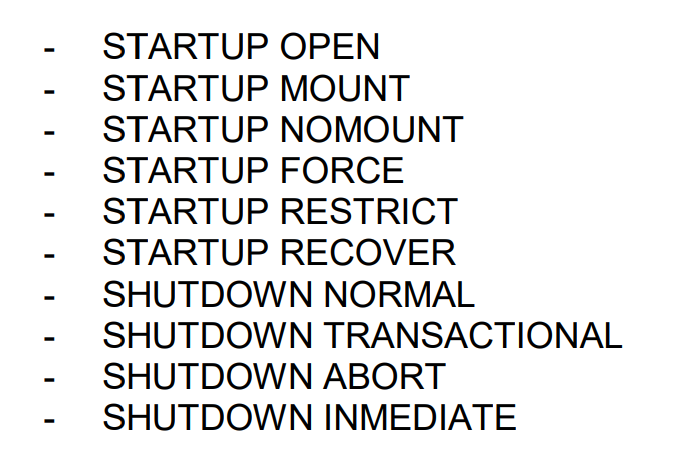
\includegraphics[width=8cm]{./Imagenes/actividad_5_1_lab_06}
	\end{center}	

	- STARTUP OPEN 
	\\Cuando inicia una base de datos, crea una instancia de esa base de datos y determina el estado de la base de datos. Monturas y abre la base de datos especificada.
	\\
	\\- STARTUP MOUNT 
	\\Monta un base de datos, pero no lo abre.
	\\
	\\- STARTUP NOMOUNT 
	\\Causa que la base de datos no se monte al inicio de la instancia 
	\\
	\\- STARTUP FORCE 
	\\Apaga la instancia actual de Oracle Database (si se est\'a ejecutando) con el modo SHUTDOWN ABORT, antes de reiniciarlo. Si la instancia actual se est\'a ejecutando y no se especifica 
	\\FORCE, se produce un error. FORCE es útil durante la depuración y en circunstancias anormales. Normalmente no debería ser usado.
	\\
	\\- STARTUP RESTRICT 
	\\Solo permite a los usuarios de Oracle Database con el privilegio del sistema RESTRICTED SESSION conectarse a la base de datos. M\'as tarde, puede usar el comando ALTER SYSTEM 
	\\para deshabilitar la caracter\'istica de sesi\'on restringida.
	\\
	\\- STARTUP RECOVER 
	\\Especifica que se debe realizar la recuperación de medios, si es necesario, antes de iniciar la instancia. STARTUP RECOVER tiene el mismo efecto que emitir el comando RECOVER
	 \\DATABASE e iniciar una instancia. Solo es posible la recuperaci\'on completa con la opci\'on RECUPERAR.
	\\La recuperaci\'on contin\'ua, si es necesario, como si AUTORECOVERY estuviera configurado en ON, independientemente de si AUTORECOVERY est\'a habilitado o no. Si no se encuentra 
	\\un archivo de registro de rehacer en la ubicaci\'on esperada, la recuperaci\'on contin\'ua como si AUTORECOVERY estuviera deshabilitado, solicit\'andole la ubicaci\'on sugerida y el nombre 
	\\de los archivos de registro posteriores que deben aplicarse.
	\\
	\\- SHUTDOWN NORMAL 
	\\NORMAL es la opci\'on predeterminada que espera que los usuarios se desconecten de la base de datos.
	\\M\'as conexiones est\'an prohibidas. La base de datos est\'a cerrada y desmontada. La instancia se apaga y no se requiere recuperaci\'on de instancias en el pr\'oximo inicio de la base de 
	\\datos.
	\\
	\\- SHUTDOWN TRANSACTIONAL 
	\\Realiza un cierre planificado de una instancia al tiempo que permite que las transacciones activas se completen primero. Evita que los clientes pierdan el trabajo sin requerir que todos 
	\\los usuarios cierren la sesi\'on.
	\\Ning\'un cliente puede iniciar una nueva transacci\'on en esta instancia. Intentar iniciar una nueva transacci\'on provoca la desconexi\'on. Despu\'es de completar todas las transacciones, 
	\\cualquier cliente que todav\'ia est\'e conectado a la instancia se desconectar\'a. Ahora la instancia se cierra como lo har\'ia si se enviara una instrucción SHUTDOWN INMEDIATA. El pr\'oximo 
	\\inicio de la base de datos no requerir\'a ningún procedimiento de recuperación de instancias.
	\\El modo LOCAL especifica un cierre transaccional solo en la instancia local, por lo que solo espera que se completen las transacciones locales, no todas las transacciones. Esto es \'util, 
	\\por ejemplo, para el mantenimiento programado de la interrupci\'on.
	\\
	\\- SHUTDOWN ABORT 
	\\Procede con el cierre m\'as r\'apido posible de la base de datos sin esperar a que finalicen las llamadas o que los usuarios se desconecten.
	\\Las transacciones no confirmadas no se revierten. Las sentencias de SQL del cliente que se est\'an procesando est\'an finalizadas. Todos los usuarios actualmente conectados a la base 
	\\de datos est\'an desconectados impl\'icitamente y el pr\'oximo inicio de la base de datos requerir\'a la recuperaci\'on de la instancia.
	\\Debe usar esta opci\'on si un proceso en segundo plano termina anormalmente.
	\\
	\\- SHUTDOWN INMEDIATE
	\\No espera a que finalicen las llamadas actuales o que los usuarios se desconecten de la base de datos.
	\\M\'as conexiones estn prohibidas. La base de datos est\'a cerrada y desmontada. La instancia se apaga y no se requiere recuperaci\'on de instancias en el pr\'oximo inicio de la base de 
	\\datos.

	

	\item . En el script lab\_02\_01.sql, se establecen privilegios de sistema, enliste los privilegios de sistema (DDL) utilizados y describa cada uno de ellos.
	\\\\- create table 
	\\- insert into
	\\- exec
	\\- begin tran
	\\- save tran
	\\- delete
	\\- select
	\\- rollback tran
	\\- alter proc
	\\- declare
	\\-  create sequence
	\\- drop sequence
	\\- create index
	\\- creatw synonym
	
	\item Enliste y describa los tipos de TableSpace que existen en Oracle.
	\\\\ existen dos tipos de tablespace :
	\\- TableSpace System	: se crea automaticamente al hacer la instalacion de oracle o al crear una BD.
	\\- TableSpace Temporales	: es aquel en el que solamente puede haber objetos temporales
	\\\\- de tipo deshacer cambios	: se utilizan para gestionar poder deshacer las transacciones incompletas.
	\\- con tamaño de bloque variable
	\\- de tipo BigFile	
	

\end{enumerate} 
